\documentclass{article}

\usepackage{graphicx}
\usepackage{amsmath}
\usepackage{amssymb}
\usepackage{siunitx}
\usepackage{hyperref} % for \url{}

% This stuff is for figures
\usepackage{float}
\DeclareGraphicsExtensions{.pdf, .png, .jpg}

\hypersetup{
    colorlinks=true,
    urlcolor=blue
}

\renewcommand{\c}[1]{\texttt{#1}}
%https://tex.stackexchange.com/questions/112932/today-month-as-text
\renewcommand{\today}{\ifnum\number\day<10 0\fi \number\day \space%
\ifcase \month \or January\or February\or March\or April\or May%
\or June\or July\or August\or September\or October\or November\or December\fi\space%
\number \year} 

\begin{document}

%\begin{flushright}
    \noindent
    Rodrigo Becerril Ferreyra\\
    CECS 361 Section 01\\
    Lab 4\\
    \today
    %30 October 2020
%\end{flushright}

%\addcontentsline{toc}{section}{Introduction}
\section{Introduction} The purpose of this lab
assignment
is to practice
implementing finite-state machines (FSMs) and modularization
of a design. Specifically, the objective of this lab assignment
is to implement a \href{https://en.wikipedia.org/wiki/Euclidean_division}
{Euclidean division} algorithm.

In short, for \(A, B \in \mathbb{Z}\) and \(B\ne0\),
there exists two unique integers \(Q\) and \(R\) such that
\begin{equation}
    A = BQ + R
\end{equation} and
\begin{equation}
    0 \le R < |B|.
\end{equation}In this lab, we are given an algorithm
and digital implementation
to find \(Q\) and \(R\) (called the quotient and remainder,
respectively); our job is to construct this implementation
from a given digital circuit:

\begin{figure}[H]
    \centering
    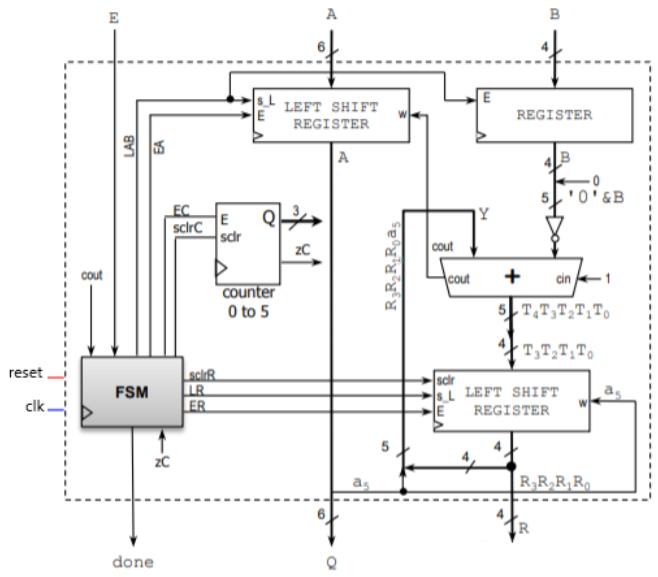
\includegraphics[height=250pt]{Images/circuit}
    \caption{Architectural schematic. (c) Oakland University, ECE department, used without permission.}
    \label{circuit}
\end{figure}

This circuit incorporates various smaller digital circuits,
such as various types of registers, counters, and a
combinatorial addition circuit. The circuit takes in
\c{A} and \c{B}, and outputs \c{Q} and \c{R}, along with a
\c{done} bit which is high when the algorithm is finished.

\section{Implementation} To start, we were given two modules to
use: one six-bit left-shift loadable register, and one
four-bit left-shift loadable register with synchronous clear.
We were required to create the following circuits
in order for the implementation to work:
\begin{itemize}
    \item a four-bit loadable register.
    \item a modulo-6 counter.
    \item a combinatorial five-bit full adder.
    \item a controller modified by a finite state machine (FSM).
\end{itemize}

After all the modules were constructed, we were tasked with
connecting them in accordance to Figure \ref{circuit}.
All sequential circuits share
\c{clk} (clock) and \c{rst} (reset) values
unless otherwise stated.

\subsection{Loadable, left-shift registers} These circuits
were given in the project description. Their functionality
is as follows: when their enable input \c{E} is high,
the value held by the register is shifted over one
place to the left, and the value at \c{w} is written
to the LSB, all on the rising edge of the clock;
when \c{E} is low, the register retains its value. The
four-bit register also has a synchronous clear input \c{s\_L}
(as opposed to the asynchronous clear input \c{rst}) which
clears the contents of the register on the rising edge
of the clock.

\subsection{Four-bit loadable register} This module was the
easiest of all to construct. It is simply a four-bit register
with an ``enable'' or ``write'' input (named \c{E}), and its
functionality is as follows: if \c{E} is low, the register
holds its current value; if \c{E} is high, the value on
its input \c{D} gets copied to its output \c{Q} on the next
rising edge of the clock.

\subsection{Modulo-6 counter} The functionality of this
circuit is as follows: internally, the circuit consists of a
two-bit register that holds the current count. When the enable
input \c{E} is high, the value of this register will increment
on the rising edge of the clock; if \c{E} is low, it will
keep its value. The register has a \c{sclr} (synchronous
clear) which clears the value of the register on the rising
edge of the clock.

When this register reaches the value of 5, the output \c{zC}
is set, and the next value the register takes on is 0. Any
other value of the register clears \c{zC} (the value of the
register is also an output (named \c{Q}), but is not used
in this design).

\subsection{Combinatorial five-bit full adder} This full
adder takes in two five-bit inputs \c{A} and \c{B} and a
one-bit input \c{cin}, and adds them together in the output vector
\c{\{cout, Sum\}}, where \c{Sum} is five bits long and \c{cout}
is a scalar. This design allows the \c{cout} to be
differentiated from the five-bit result of the summation,
allowing it to be separated and sent different directions.

\subsection{Controller} Last but not least, the controller,
modeled by a FSM, was the most complex part of this lab.
The controller can have three states
(if modeled by a Mealy machine)
or six states (if modeled by a Moore machine). Below is a
comparison of the state diagram of the FSM as modeled
by different types of machines.

\begin{figure}[H]
    \centering
    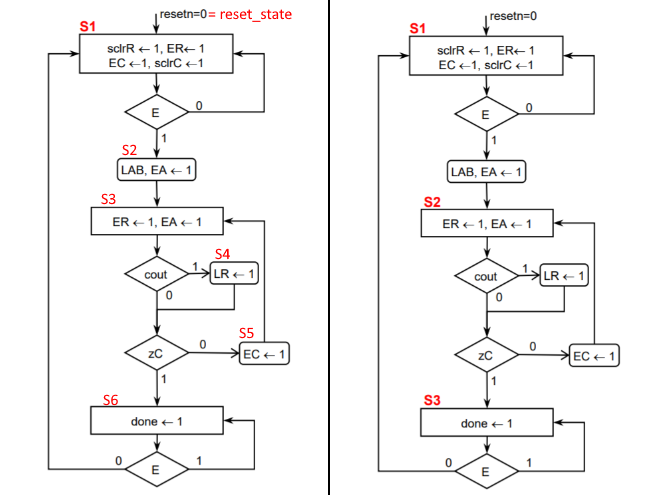
\includegraphics[width=\textwidth]{Images/FSM_diagram.png}
    \caption{A Moore machine (left) vs a Mealy machine (right). (c) Jos\'e Aceves \& Amin Rezaei.}
    \label{statediagram}
\end{figure}

Its outputs
drive the inputs to almost all of the other circuits
(excluding the adder). Its inputs are driven by a combination
of user inputs and internal wires from the outputs of other
circuits.

At first, to simplify the design process, I designed the
controller using an Moore machine model, as I find them
easier to implement. It was very helpful
in choosing the format to describe the controller in
the Verilog language.
However, I ran into trouble due to the fact that
a Moore machine requires double the amount of states
with respect to a Mealy machine, and therefore you need
double the amount of bits to encode all states. My trouble
stemmed from the fact that I was using two bits to encode
my states instead of the required three. Once that was fixed,
the controller ran as planned. Below are the block diagrams
of the defective Moore machine, working Moore machine, and
Mealy machine implementations of the controller.

\begin{figure}[H]
    \centering
    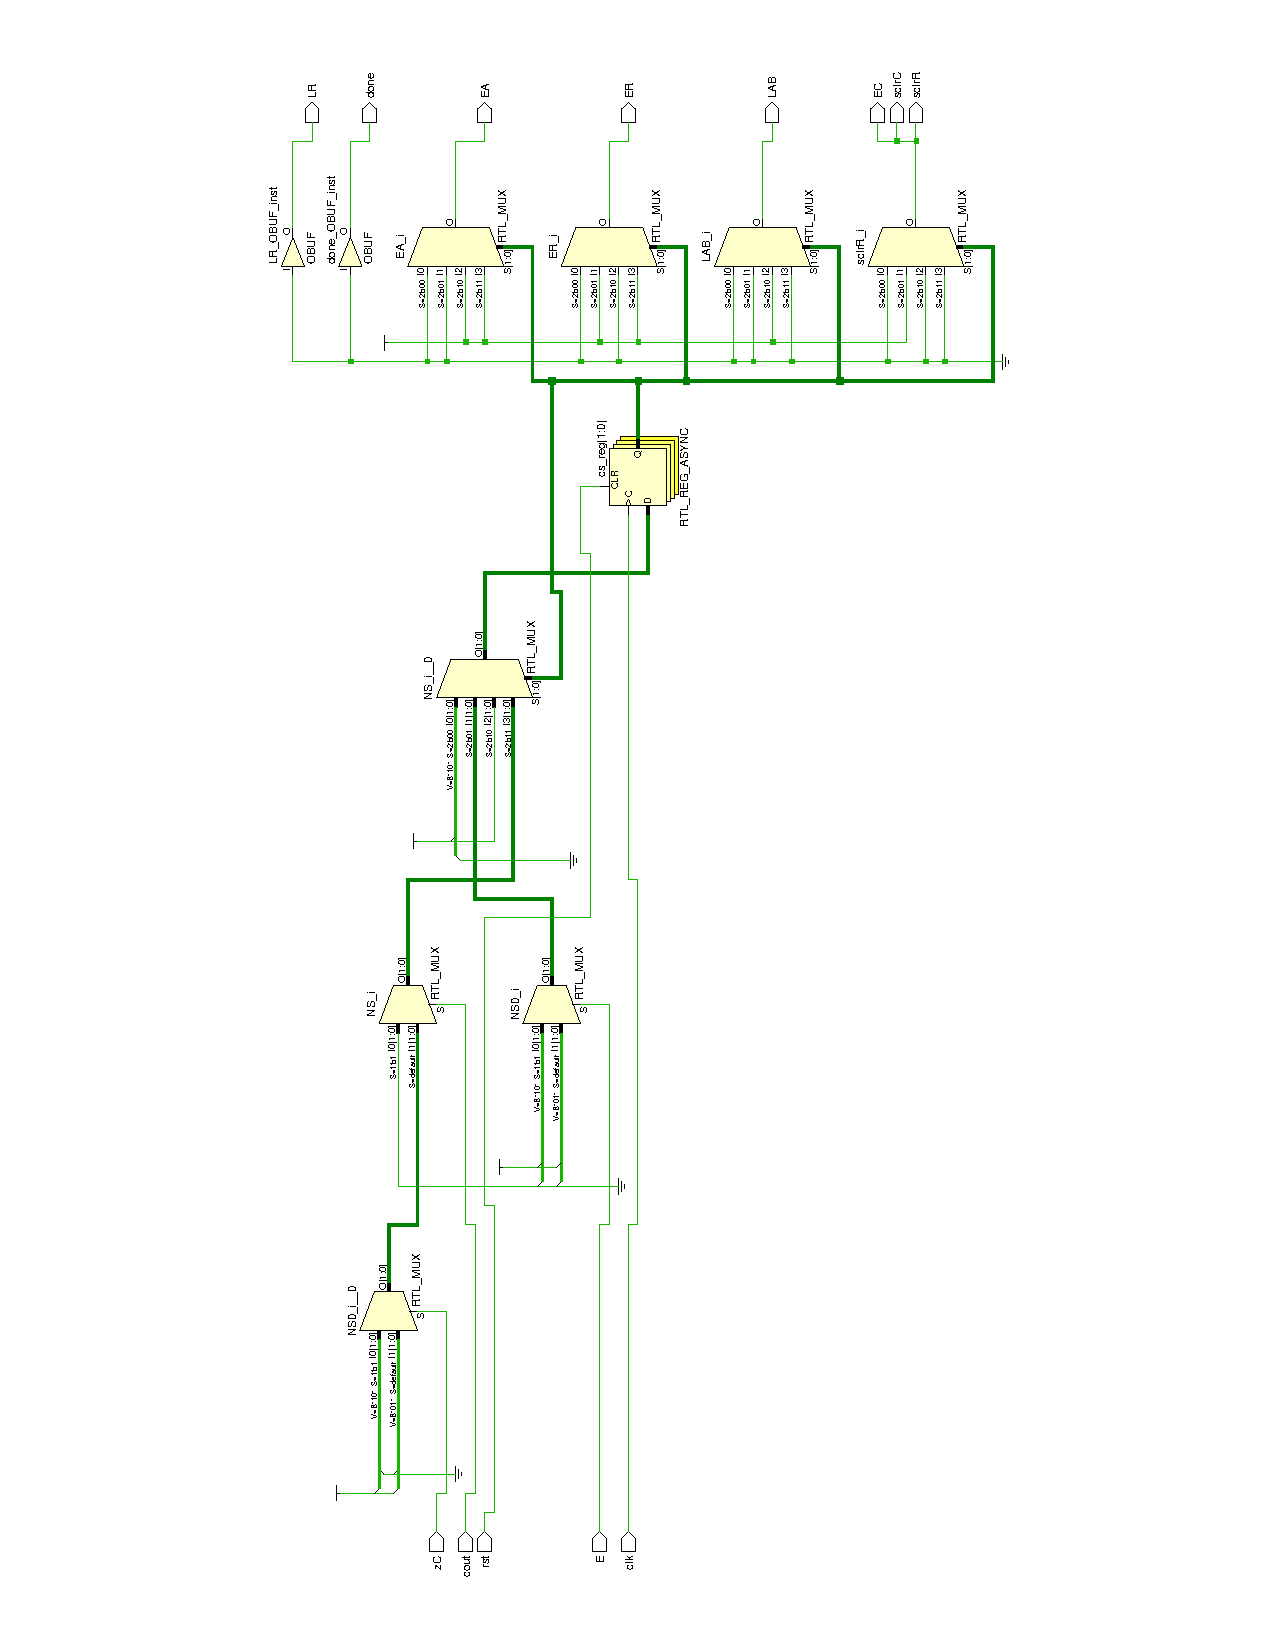
\includegraphics[height=\textwidth, angle=-90]{Images/schematic1}
    \caption{Defective Moore machine implementation.}
    \label{blockdiagram:moore1}
\end{figure}
\begin{figure}[H]
    \centering
    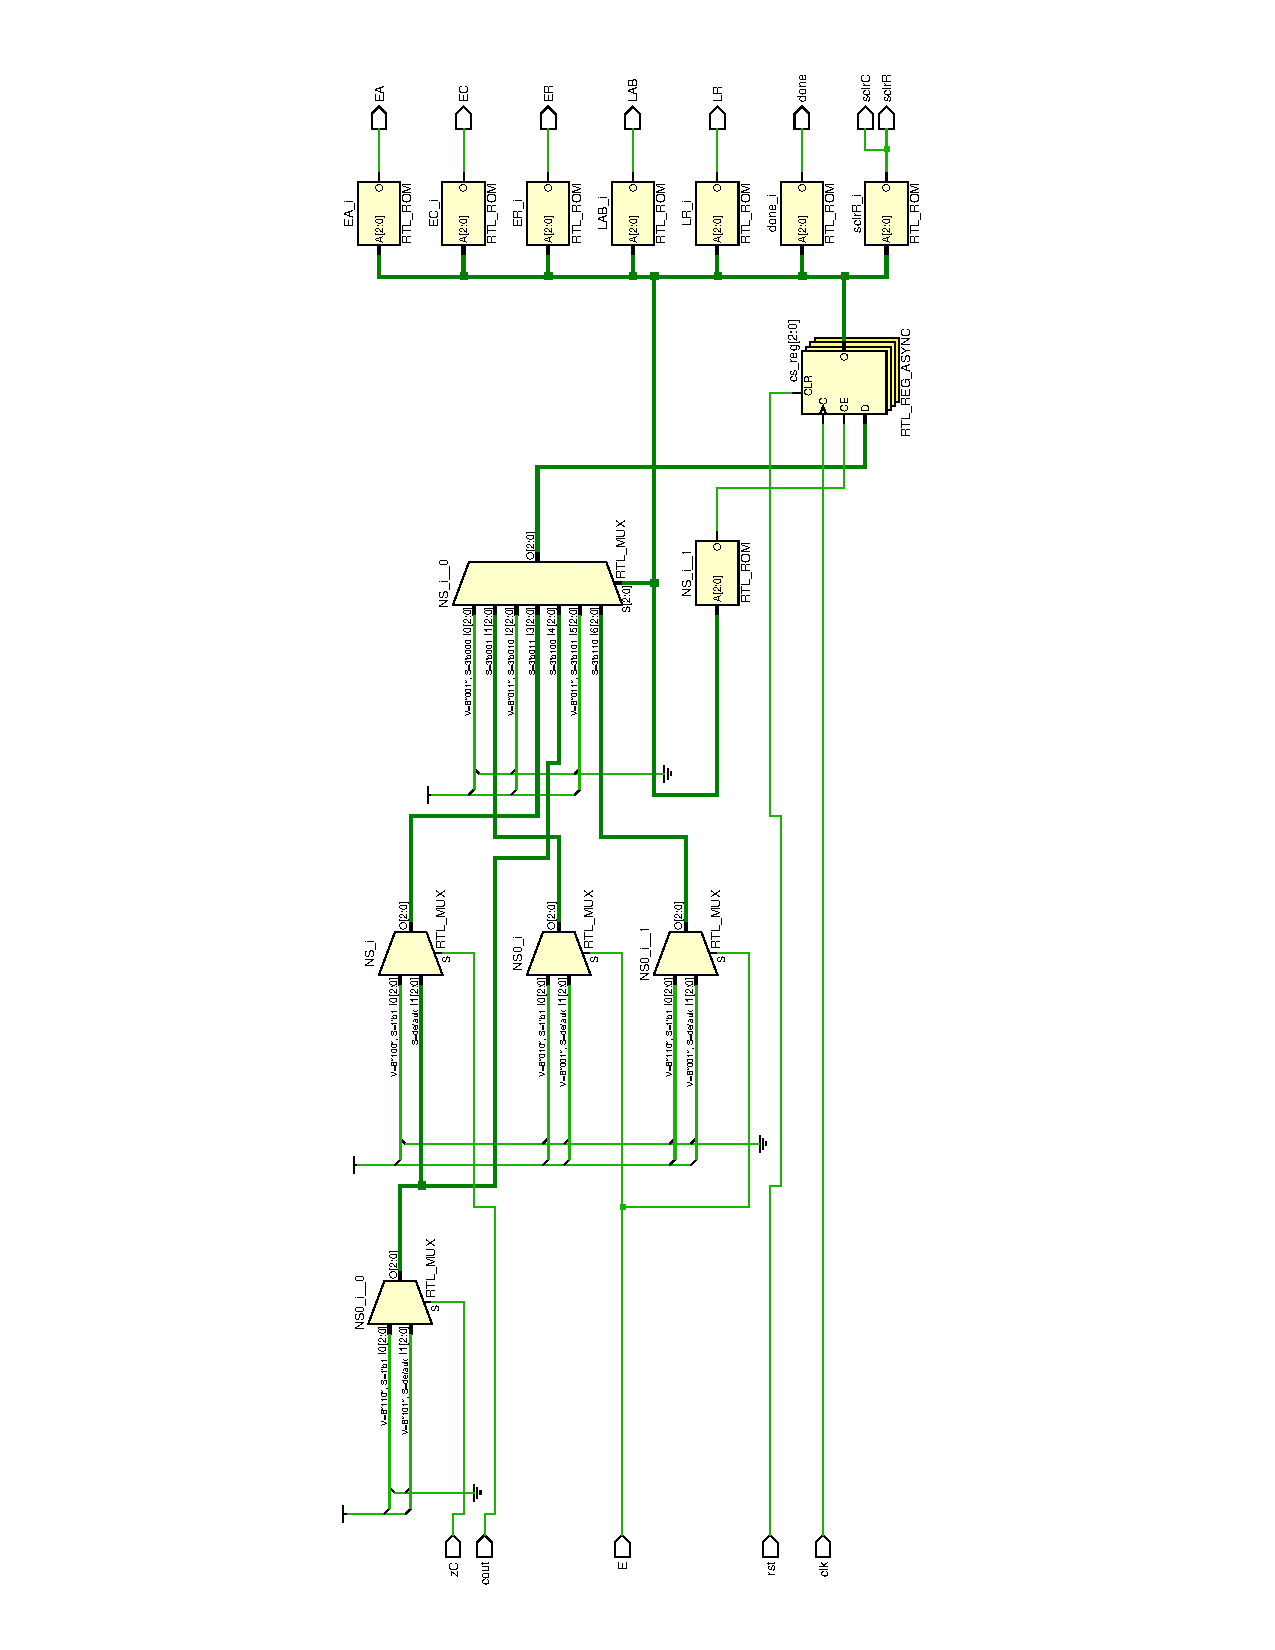
\includegraphics[height=\textwidth, angle=-90]{Images/schematic2}
    \caption{Working Moore machine implementation.}
    \label{blockdiagram:moore2}
\end{figure}
\begin{figure}[H]
    \centering
    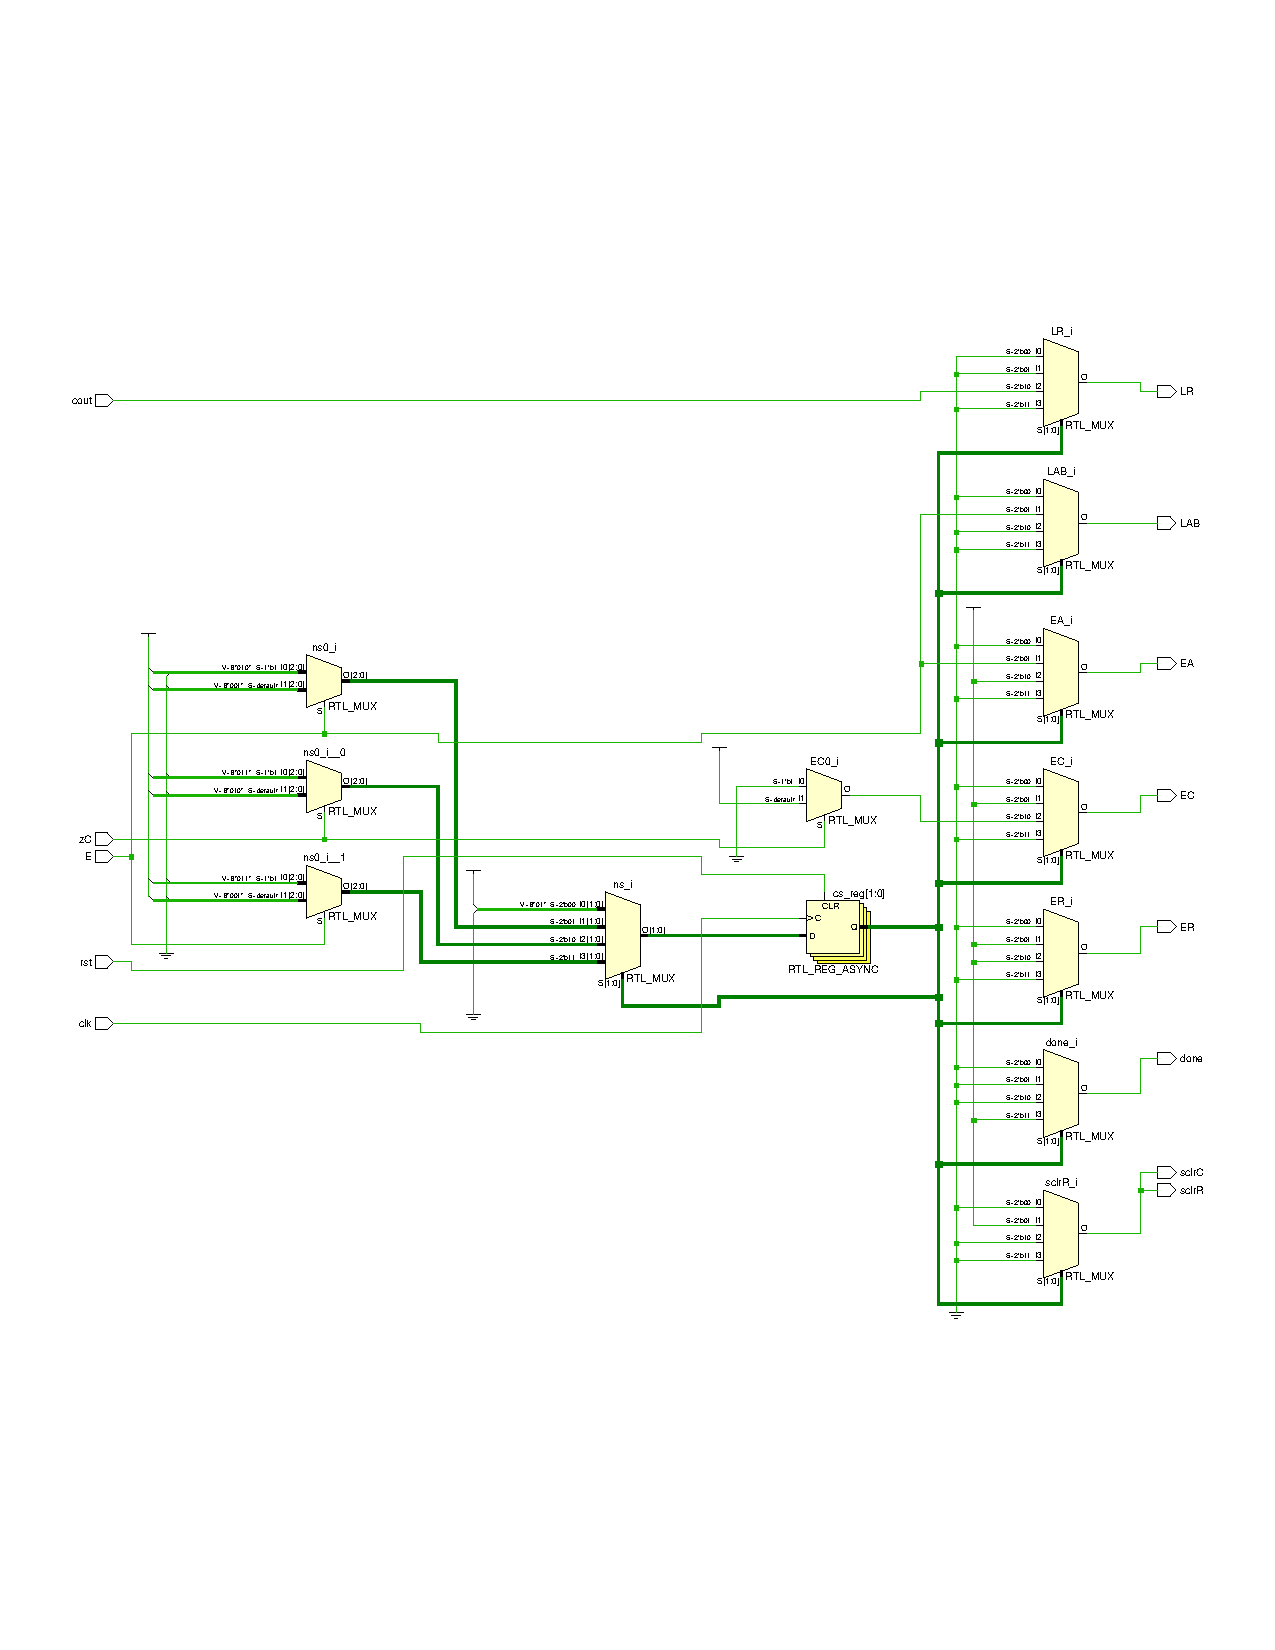
\includegraphics[width=\textwidth]{Images/schematic_final}
    \caption{Mealy machine implementation.}
    \label{blockdiagram:mealy}
\end{figure}

(The above diagrams are vector images, so feel free to zoom
in if viewing on a computer.)
Note that Figure \ref{blockdiagram:moore1} has various outputs
stuck at zero (connected to ground);
this is a clear indication that certain states
cannot be reached (namely those with state encodings greater
than 3). The working Moore machine in Figure
\ref{blockdiagram:moore2} fixes this issue, but introduces
\c{RTL\_ROM} blocks. Figure \ref{blockdiagram:mealy} gets
rid of these blocks and has an easy-to-follow
flow. In the end, I decided to use the Mealy design,
due to the fact that it did not include any \c{RTL\_ROM}
blocks.

\subsection{Top-level module} The top-level design was as
simple as following the design layed out in Figure
\ref{circuit}; in the case of implied connections such as
\c{cout}, like-named wires are connected. Below is
a diagram of the final top-level circuit; feel free to
compare it to the circuit in Figure \ref{circuit}.

\begin{figure}[H]
    \centering
    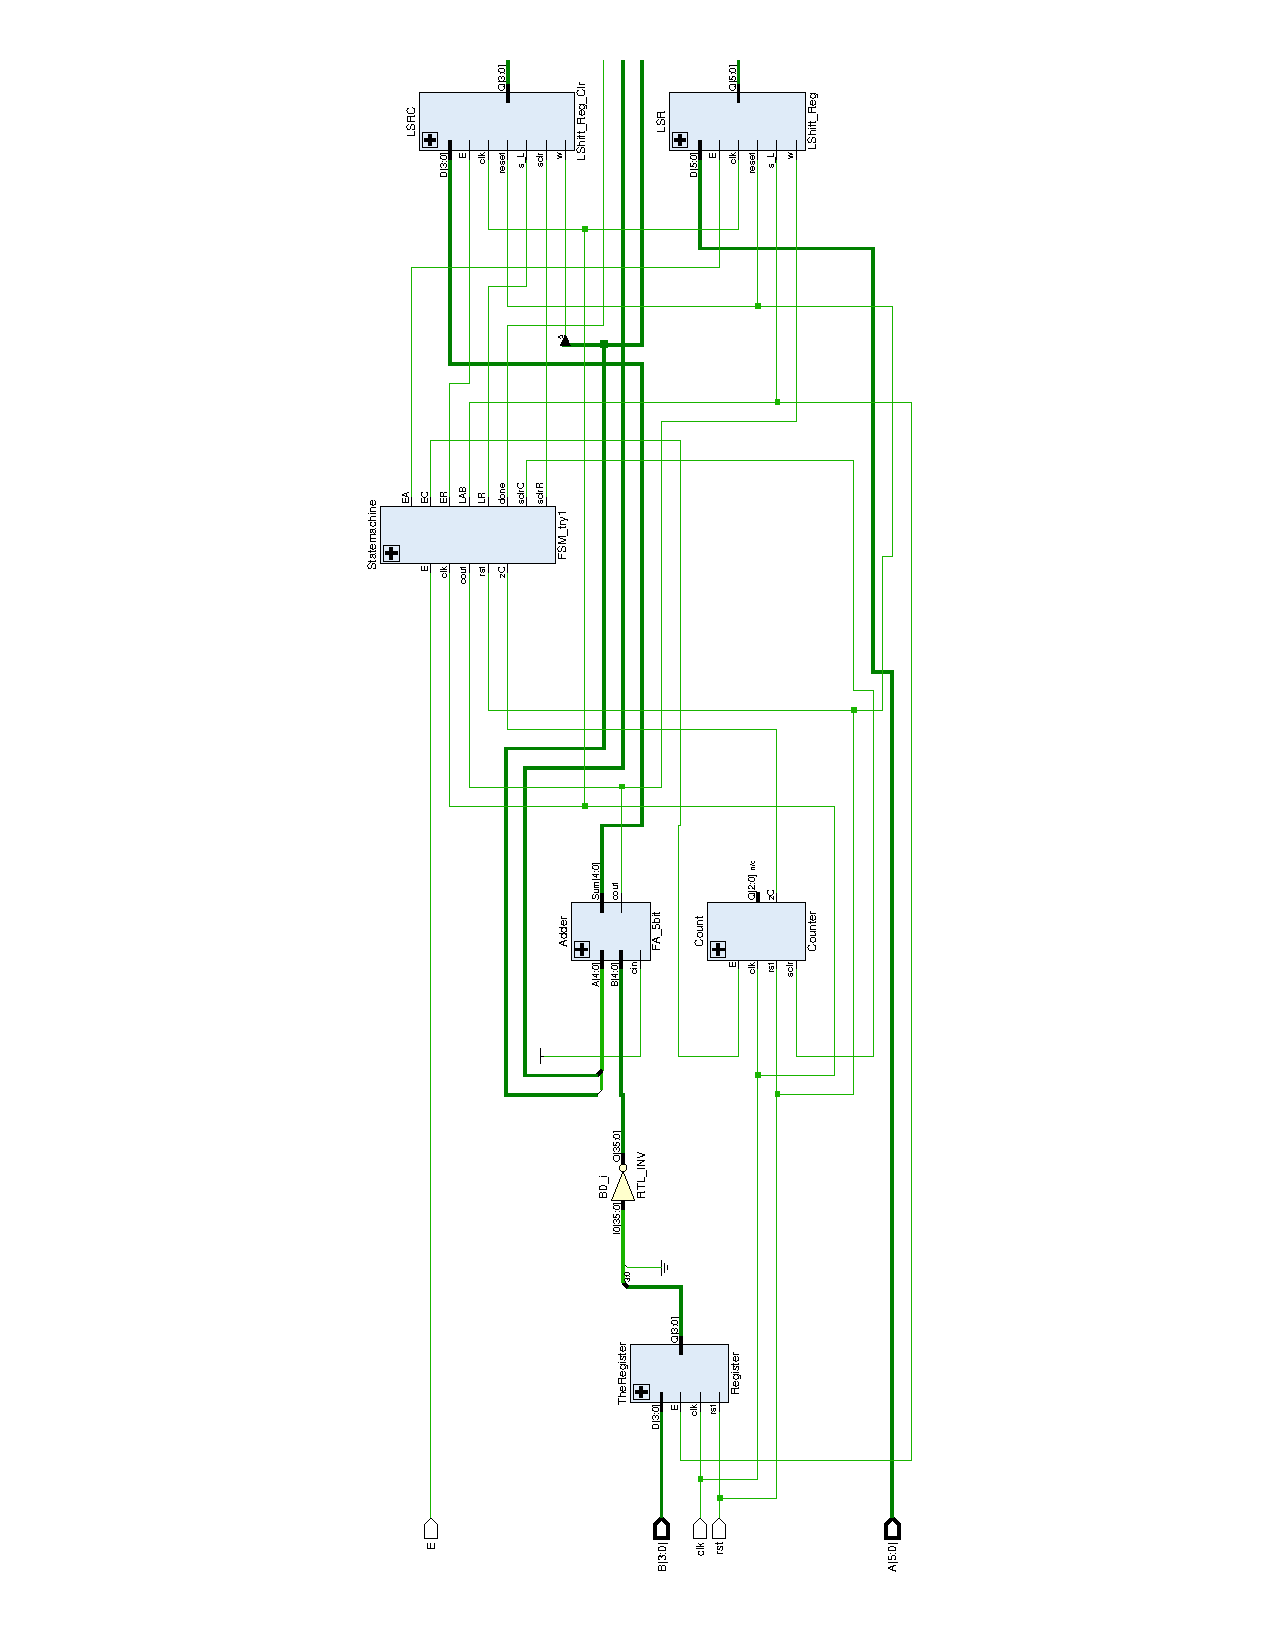
\includegraphics[height=\textwidth, angle=-90]{Images/schematic_top}
    \caption{Top-level diagram.}
    \label{blockdiagram:top}
\end{figure}

\section{Testing and Verification} Testing was performed at
each step of the designing process: after a circuit was
completed, it was verified for correctness. Below is a
compilation of waveform outputs of all the circuits
that were created. Note that the given circuits were not
tested and taken to be correct.

\subsection{Four-bit loadable register}
\begin{figure}[H]
    \centering
    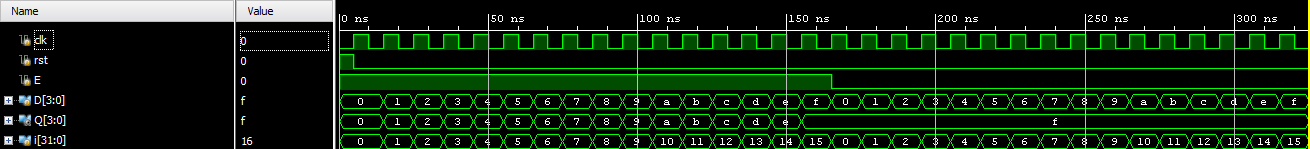
\includegraphics[width=\textwidth]{Images/Register_waveform}
    \caption{Loadable register testing.}
    \label{test:register}
\end{figure}

In this test, the enable input is set for 16 clock cycles, and
as one can see, the value gets copied from \c{D} to \c{Q}
on the rising edge of the clock, as a register should.
However, when \c{E} is cleared, the register retains its
value. This is the desired behavior.

\subsection{Modulo-6 counter}
\begin{figure}[H]
    \centering
    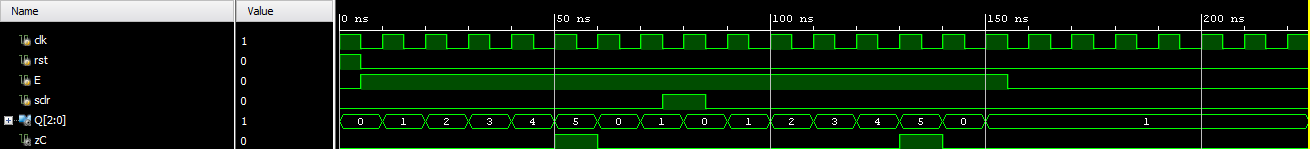
\includegraphics[width=\textwidth]{Images/Counter_waveform}
    \caption{Modulo-6 testing.}
    \label{test:counter}
\end{figure}

In this test, the enable input \c{E} is turned on, allowing
the counter to count. As specified, when the value of the
counter \c{Q} reaches 5, \c{zC} is set, and the next value
of \c{Q} is 0. At about \SI{75}{ns}, \c{sclr} is asserted,
clearing the contents of the register on the rising edge of
the clock. Later in the test, \c{E} is cleared, stopping the
counter and keeping the value constant. This is the
desired behavior.

\subsection{Combinatorial five-bit full adder}
\begin{figure}[H]
    \centering
    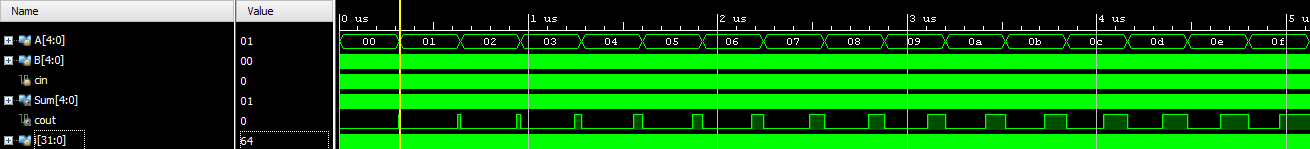
\includegraphics[width=\textwidth]{Images/Adder_waveform_full}
    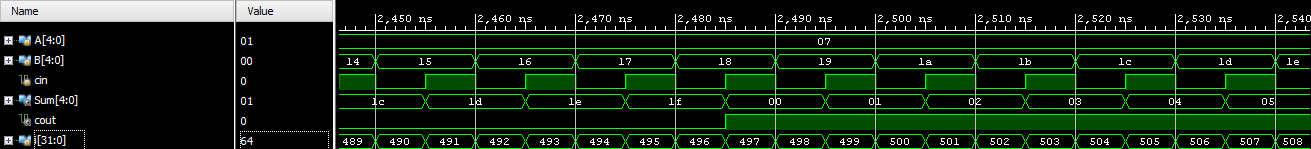
\includegraphics[width=\textwidth]{Images/Adder_waveform_zoom}
    \caption{Five-bit adder testing.}
    \label{test:adder}
\end{figure}

The first image in Figure \ref{test:adder} shows the full
waveform in a compressed format, while the second image
shows a portion of this waveform for clarity.

In this test, the values of \c{A} and \c{B} were looped through
iteratively, which is guaranteed to test all possible values
for these two inputs. The output is then verified with the
expected result. This is the desired behavior.

\subsection{Controller}
\begin{figure}[H]
    \centering
    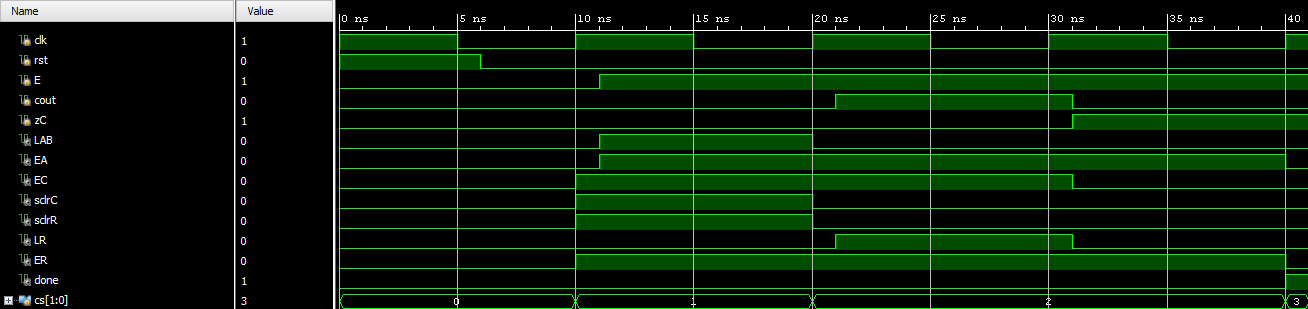
\includegraphics[width=\textwidth]{Images/FSM_waveform}
    \caption{Controller testing.}
    \label{test:controller}
\end{figure}

In this test, all distinct combinations of possible outputs
were tested; note that the bottommost signal in this
waveform represents the internal state of the controller,
is neither an input nor an output, and is only included
for clarity.

The test follows the Mealy model FSM as described in Figure
\ref{statediagram}, and has been verified to be consistent
with all outputs.

\subsection{Top-level module}
\begin{figure}[H]
    \centering
    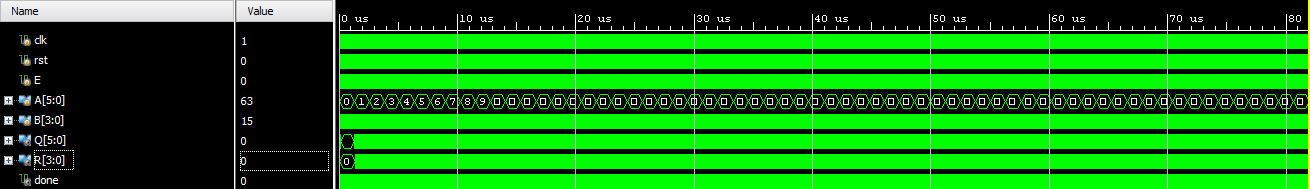
\includegraphics[width=\textwidth]{Images/top_waveform_full}
    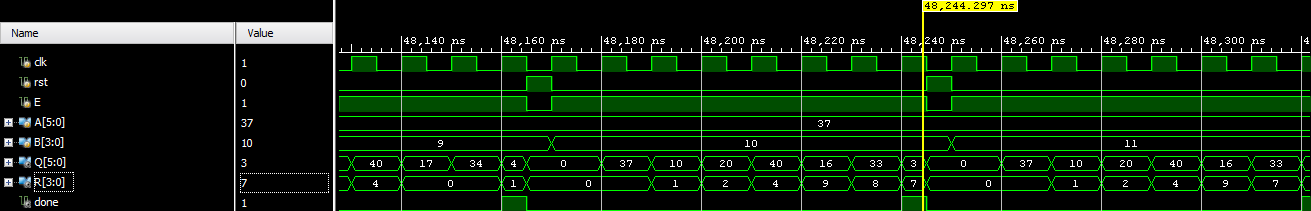
\includegraphics[width=\textwidth]{Images/top_waveform_zoom}
    \caption{Top-level module testing.}
    \label{test:top}
\end{figure}

The first image in Figure \ref{test:top} shows the full
waveform in a compressed format, while the second image
shows a portion of this waveform for clarity. Note that
results are only valid when \c{done} is set.

Extensive self-checking testing was used for this test. This
means that each result is checked with its expected value;
therefore, if any calculated value is different from the
expected value, the test will print a warning to the console.
No negative warning was printed to the console during the
testing of this module.

The way the testing was performed is as follows: the inputs
\c{A} and \c{B} are assigned iteratively, making sure that
no value is not assigned. Next, the test waits until the
\c{done} bit is raised, because as stated earlier, the
result is not valid unless \c{done} is high. At this point,
the result is checked with the expected result:
the desired quotient is calculated using \c{A/B}, and
the desired remainder is calculated using \c{A\%B}.
The test then
asserts a reset and moves on to the next test. In Figure
\ref{test:top}, the result shown is
\[37 = 10\times3 + 7,\] a true statement.

It is interesting to note what happens when the divisor is
zero; in this case, Euclidean division is not defined. What
we get is the following:

\begin{figure}[H]
    \centering
    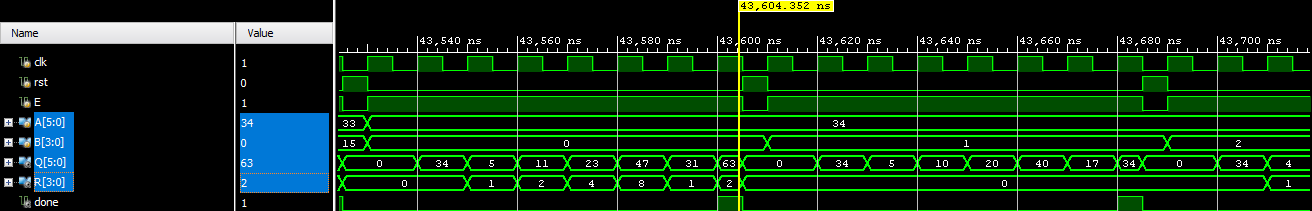
\includegraphics[width=\textwidth]{Images/top_waveform_zero}
    \caption{Division by zero example.}
    \label{test:top_zero}
\end{figure}

As we can see, the result we are getting is
\[ 34 = 0 \times 63 + 2 \], which is not a true statement.

\section{Conclusion} This lab has taught me that,
unlike implementing a multiplication circuit, implementing
a division circuit is more complex, as it needs to be
sequential instead of combinatorial, and it requires more
internal parts to do its work. The circuit also needs to
take more time to calculate its result (several clock cycles
worth of time, depending on the values being calculated),
instead happening almost instantly as is with the
multiplier circuit.

\pagebreak

\section{Media}

Below are images of the board running the test depicting
\begin{equation*}
    37 = 10\times3 + 7.
\end{equation*} The two images are the same, but the LEDs
are visible in the first image, and the switches are visible
in the second image.

\begin{figure}[H]
    \centering
    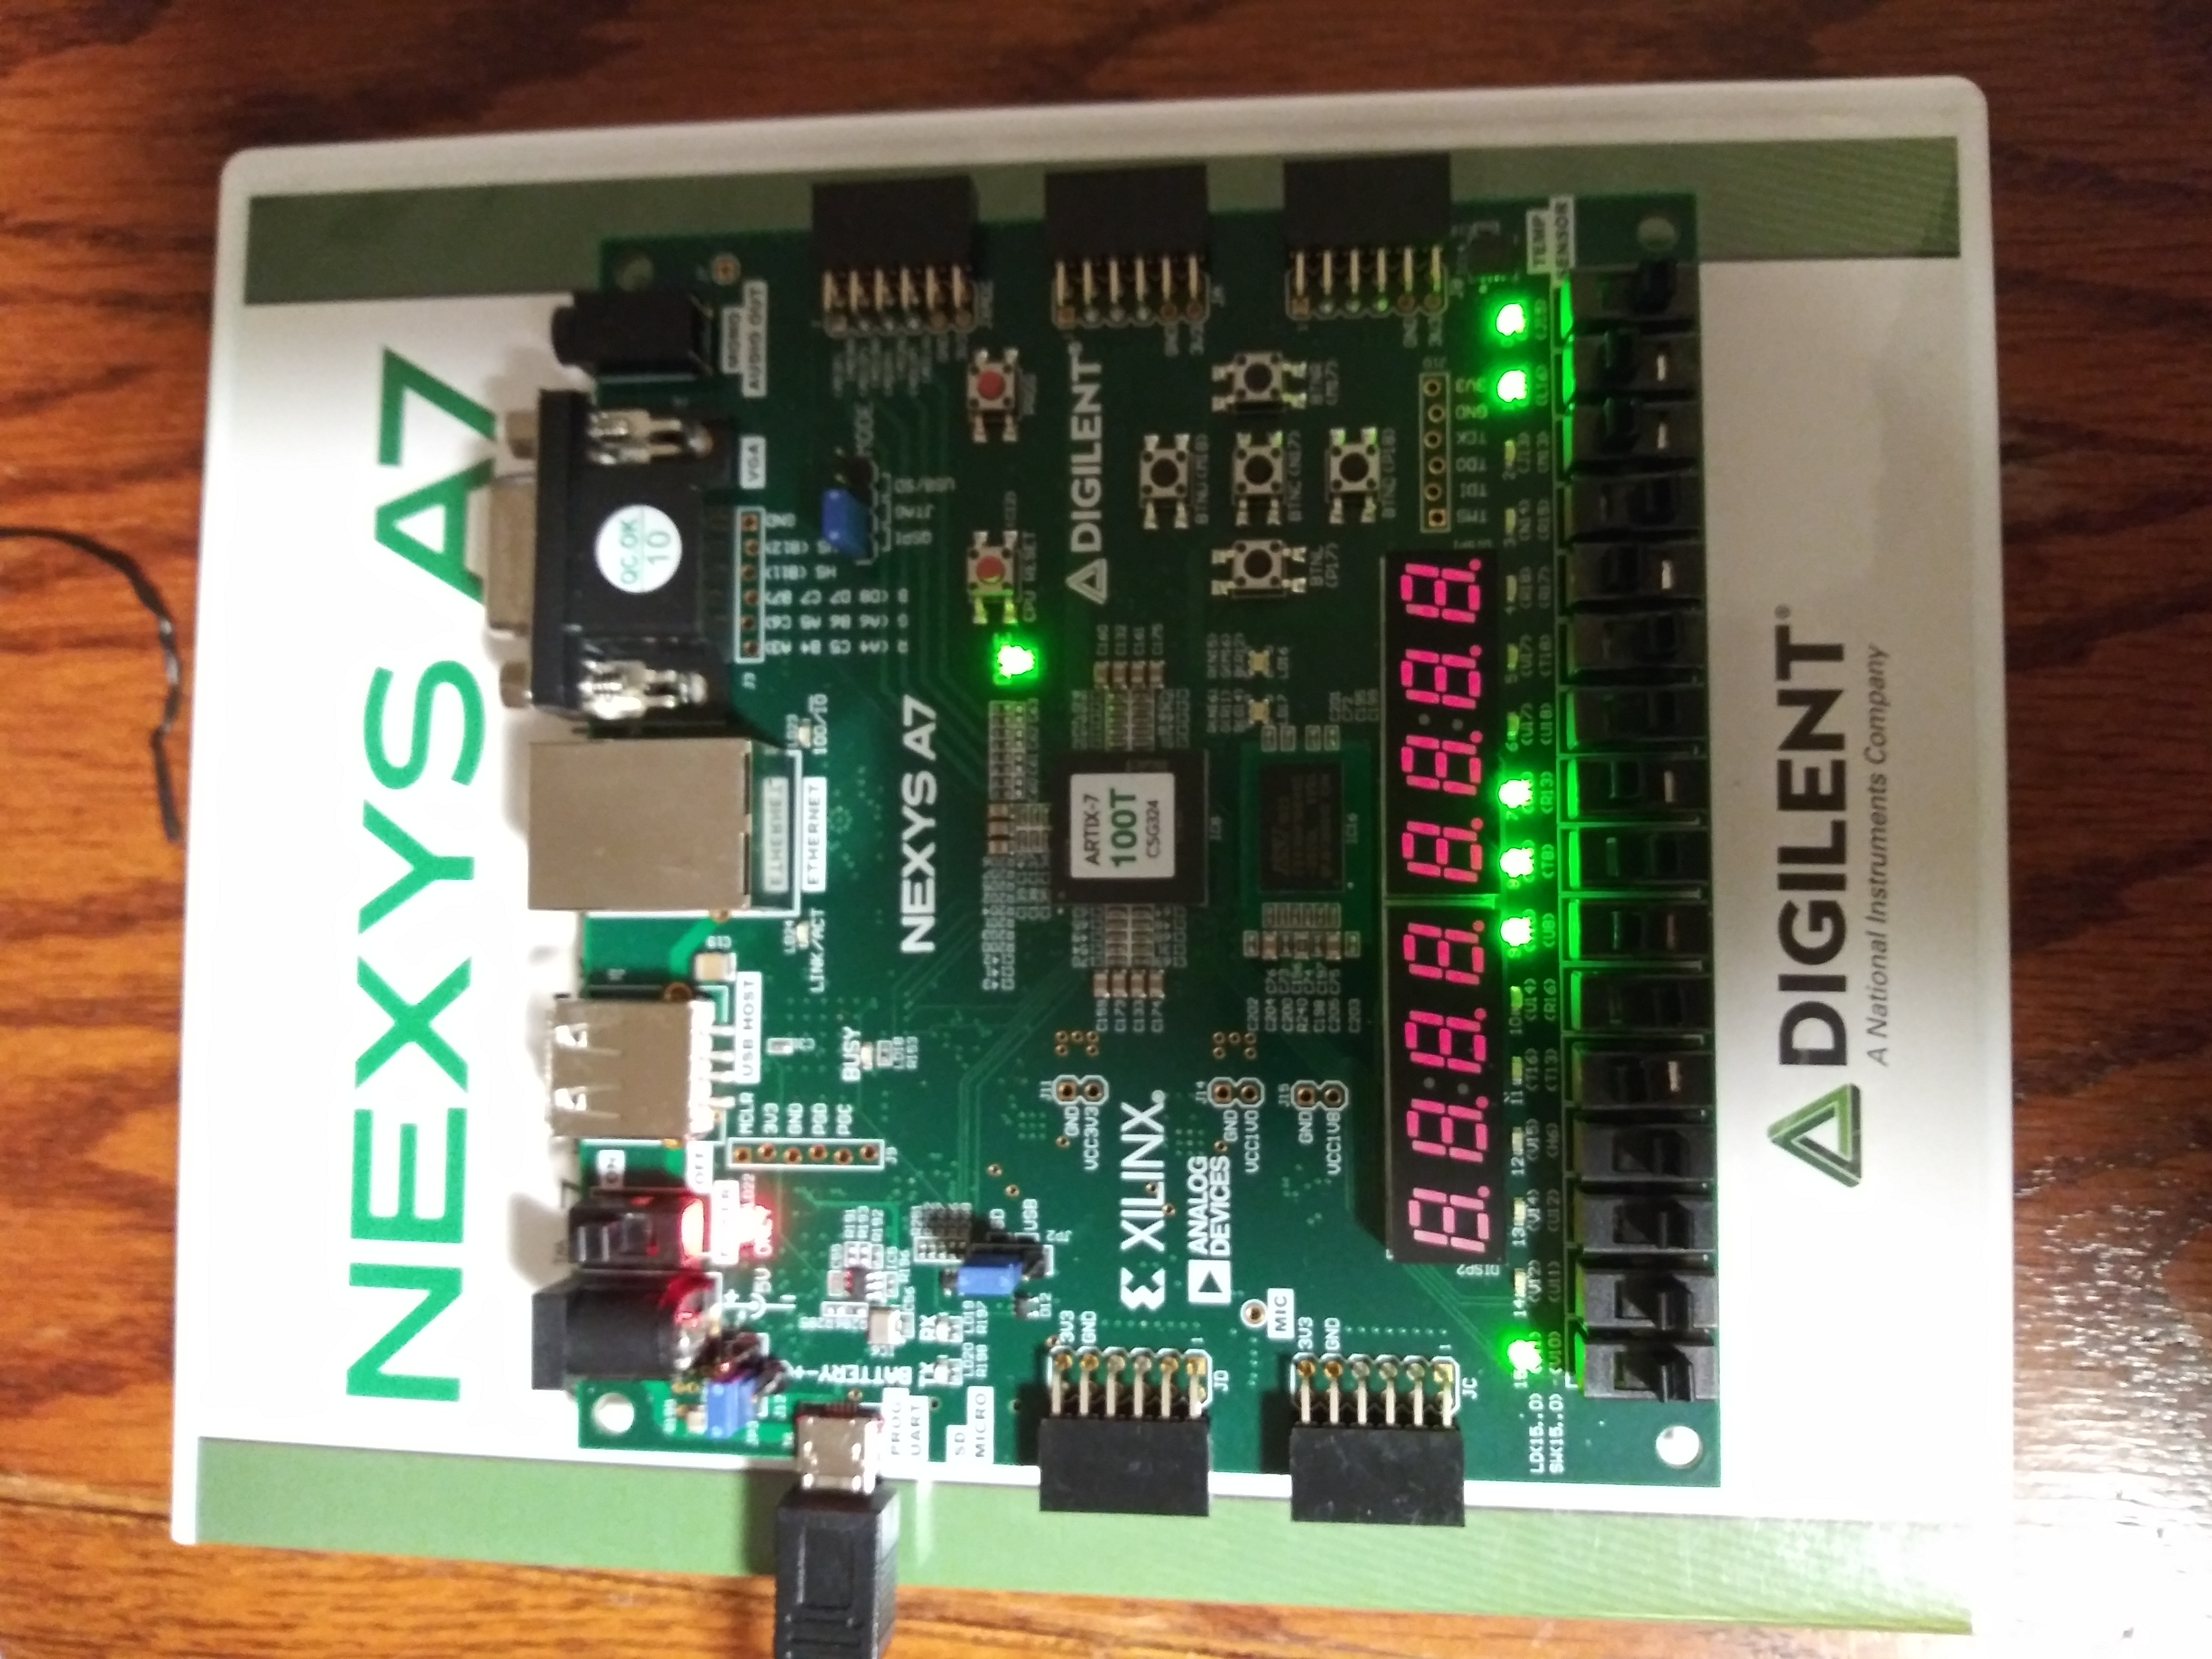
\includegraphics[width=\textwidth]{Images/20201031_043059}
    \includegraphics[width=\textwidth]{Images/20201031_043126}
    \caption{Real-time board test images.}
    \label{board}
\end{figure}

\end{document}
